\documentclass[12px]{article}

\title{Lezione 3 Fisica Generale 1}
\date{2024-10-04}
\author{Federico De Sisti}

\usepackage{amsmath}
\usepackage{amsthm}
\usepackage{mdframed}
\usepackage{amssymb}
\usepackage{nicematrix}
\usepackage{amsfonts}
\usepackage{tcolorbox}
\tcbuselibrary{theorems}
\usepackage{xcolor}
\usepackage{cancel}

\newtheoremstyle{break}
  {1px}{1px}%
  {\itshape}{}%
  {\bfseries}{}%
  {\newline}{}%
\theoremstyle{break}
\newtheorem{theo}{Teorema}
\theoremstyle{break}
\newtheorem{lemma}{Lemma}
\theoremstyle{break}
\newtheorem{defin}{Definizione}
\theoremstyle{break}
\newtheorem{propo}{Proposizione}
\theoremstyle{break}
\newtheorem*{dimo}{Dimostrazione}
\theoremstyle{break}
\newtheorem*{es}{Esempio}

\newenvironment{dimo}
  {\begin{dimostrazione}}
  {\hfill\square\end{dimostrazione}}

\newenvironment{teo}
{\begin{mdframed}[linecolor=red, backgroundcolor=red!10]\begin{theo}}
  {\end{theo}\end{mdframed}}

\newenvironment{nome}
{\begin{mdframed}[linecolor=green, backgroundcolor=green!10]\begin{nomen}}
  {\end{nomen}\end{mdframed}}

\newenvironment{prop}
{\begin{mdframed}[linecolor=red, backgroundcolor=red!10]\begin{propo}}
  {\end{propo}\end{mdframed}}

\newenvironment{defi}
{\begin{mdframed}[linecolor=orange, backgroundcolor=orange!10]\begin{defin}}
  {\end{defin}\end{mdframed}}

\newenvironment{lemm}
{\begin{mdframed}[linecolor=red, backgroundcolor=red!10]\begin{lemma}}
  {\end{lemma}\end{mdframed}}

\newcommand{\icol}[1]{% inline column vector
  \left(\begin{smallmatrix}#1\end{smallmatrix}\right)%
}

\newcommand{\irow}[1]{% inline row vector
  \begin{smallmatrix}(#1)\end{smallmatrix}%
}

\newcommand{\matrice}[1]{% inline column vector
  \begin{pmatrix}#1\end{pmatrix}%
}

\newcommand{\C}{\mathbb{C}}
\newcommand{\K}{\mathbb{K}}
\newcommand{\R}{\mathbb{R}}


\begin{document}
	\maketitle
	\newpage
	\section{Cinematica: Punto Materiale}
	Astrazione che usiamo per descrivere un corpo, non ci interessa la posizione di ogni singola parte del corpo, ma semplicemente la sua posizione nella sua compattezza.
	\subsection{Legge Oraria}
	La legge oraria è una funzione che restituisce la posizione del nostro punto dato un istante di tempo
	\[
	\overrightarrow{r}(t_1) = (x(t_1),y(t_1),z(t_1))
	.\] 
	\[
		x(t_1) = r_x(t_1) \ \ \ \text {si intende la coordinata $x$ al tempo $t_1$}
		$
	.\] 
	\textbf{Esempio}\\
	%TODO ALLIGNEA BENE
\begin{aligned}
		&t_1 \ x(t_1)\\
		&\vdots\\
		&t_n x(t_n)
	\end{aligned}\\
	\text{} \hspace{100px}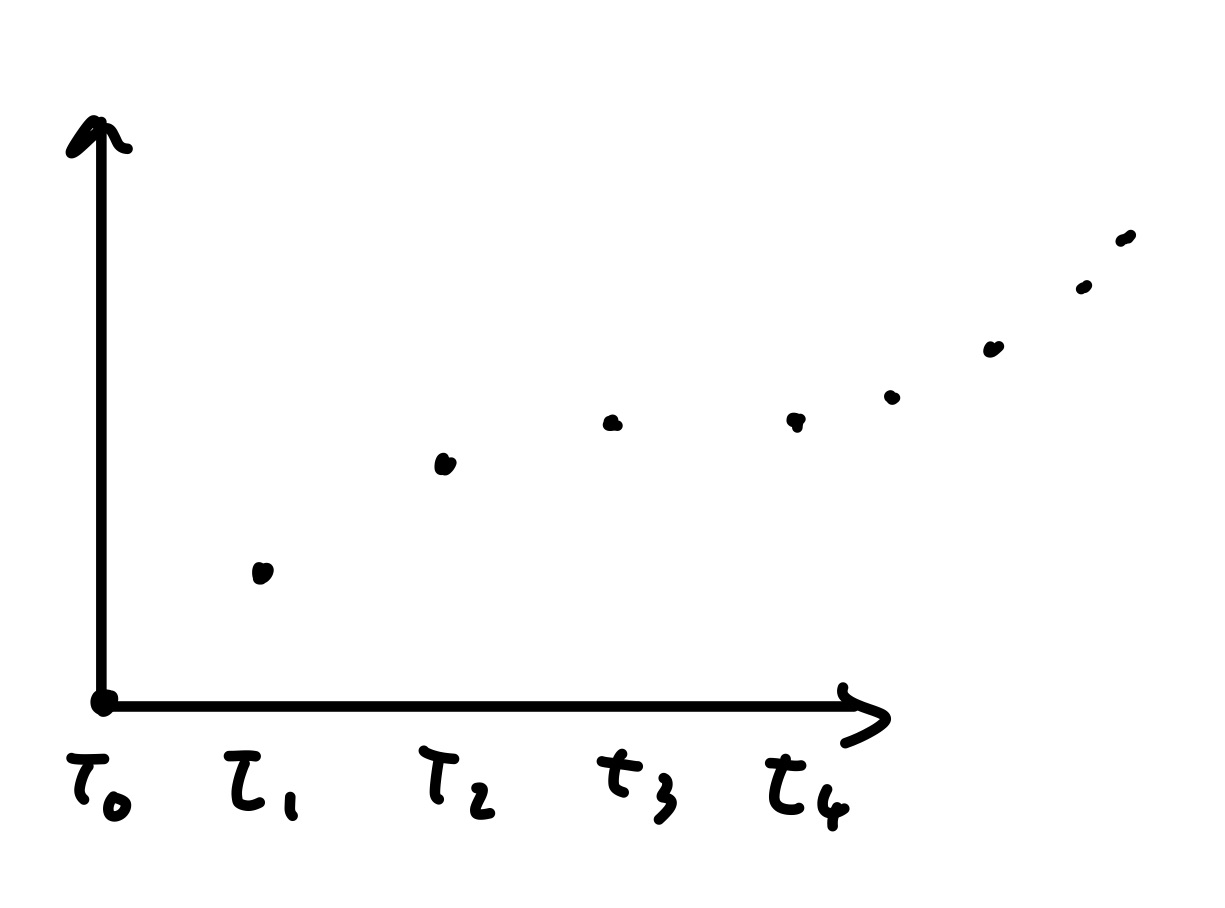
\includegraphics[scale=0.1]{grafico_1.jpeg} \ \\
	In questo grafico abbiamo i valori misurati, cerchiamo di approssimarlo ad una funzione con meno  parametri possibili con meno parametri possibili. Proviamo a descrivere ora il moto
	\[
	\begin{cases}
		x(t) = at \ \ \ \ \ \ t <t_3\\
		x(t) = \text{const}\ \  t_3\leq t<t_4\\
		x(t) = a t^2 \ \ \ \ \ \ t_4\leq  t
	\end{cases}
	.\] 
dove la prima costante ha dimensione $\displaystyle\frac l t$ e la seconda  $\displaystyle\frac l {t^2}$\\
\newpage
\subsection{Velocità}
La velocità è la variazione dello spazio nel tempo, ora definiamo velocità media e istantanea
\[
	\overrightarrow{v_m}_{[t_1,t_2]} := \frac{\overrightarrow{r}(t_2) - \overrightarrow{r}(t_1)}{t_2 - t_1}
.\] 
\[
	\overrightarrow{v}(t) = \lim_{t \rightarrow t_1} \overrightarrow{v_m}_{[t,t_1]} = \frac {d \overrightarrow{r}(t_1)}{dt}
.\] 
Quindi
\[\frac {d \overrightarrow{v}(t_1)}{dt} = \left( \frac {d x(t_1)}{dt},\frac {d y(t_1)}{dt},\frac {d z(t_1)}{dt}\right)
.\] 
\[
	\overrightarrow{v}(t) = \lim_{\Delta t \rightarrow 0}\frac{\Delta \overrightarrow{x}}{\Delta t}
.\] 
\subsection{Accelerazione}
Variazione della velocità in un determinato intervallo di tempo\\
\[
	\overrightarrow{a_m}_{[t_1,t_2]} = \frac{\overrightarrow{v_1}(t_1) + \overrightarrow{v_2}(t_2)}{t_2 - t_1}
.\] 
\[
	\overrightarrow{a}(t) = \lim_{t \rightarrow t_1} \overrightarrow{a_m}_{[t,t_1]} = \frac {d \overrightarrow{v}(t_1)}{dt}
.\] 
\[\frac {d \overrightarrow{v}(t_1)}{dt} = \left( \frac {d v_x(t_1)}{dt},\frac {d v_y(t_1)}{dt},\frac {d v_z(t_1)}{dt}\right)
.\] 
\[
	\overrightarrow{a}(t) = \lim_{\Delta t \rightarrow 0}\frac{\Delta \overrightarrow{v}}{\Delta t}
.\] 
\textbf{Esempio:}\\
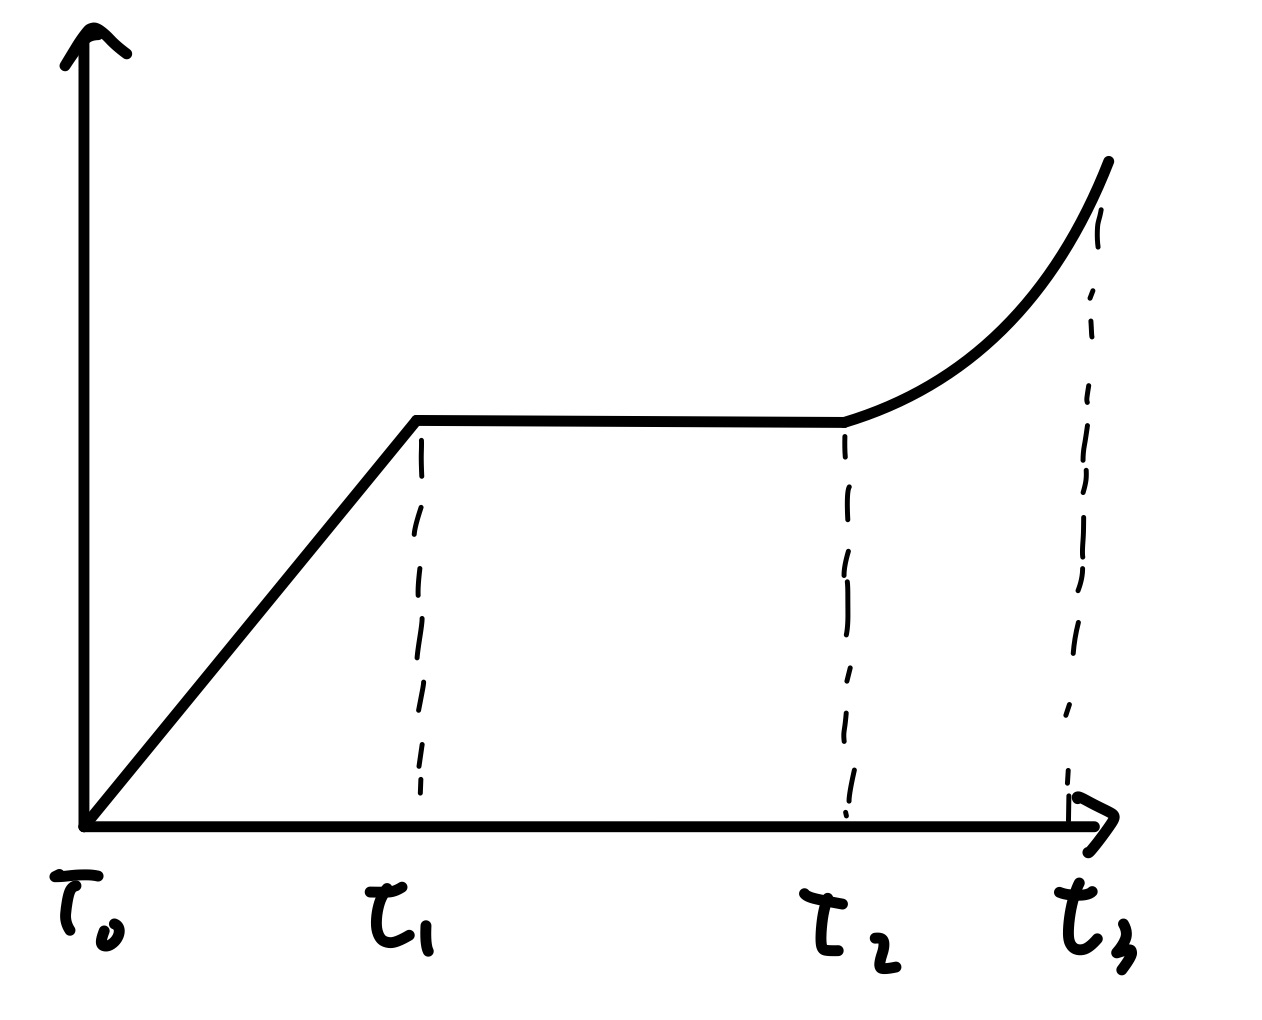
\includegraphics[scale=0.1]{grafico_2}\\
	\[
	\begin{cases}
		x(t) = at \ \ \ \ \ \ t <t_3\\
		x(t) = \text{const}\ \  t_3\leq t<t_4\\
		x(t) = a t^2 \ \ \ \ \ \ t_4\leq  t
	\end{cases}
	.\] 
	$v(t) = 2a(t - t_4) \ \ t \geq t_4$\\
	\[
		\overrightarrow{a}(t) = \frac{d \overrightarrow{v}(t)}{dt} = \frac {d v(t)}{dt} \hat v (t) + \overrightarrow{\omega_v}(t) \times \overrightarrow{v}(t)
	.\] 
	Dove $\displaystyle\frac {d v(t)}{dt} \hat v (t) = \overrightarrow{a}_t$ è la velocità tangenziale e $\overrightarrow{\omega_v}(t) \times \overrightarrow{v}(t) = \overrightarrow{a}_n$ è la velocità normale\\
	\subsection{Moto circolare}
	\begin{center}
		
	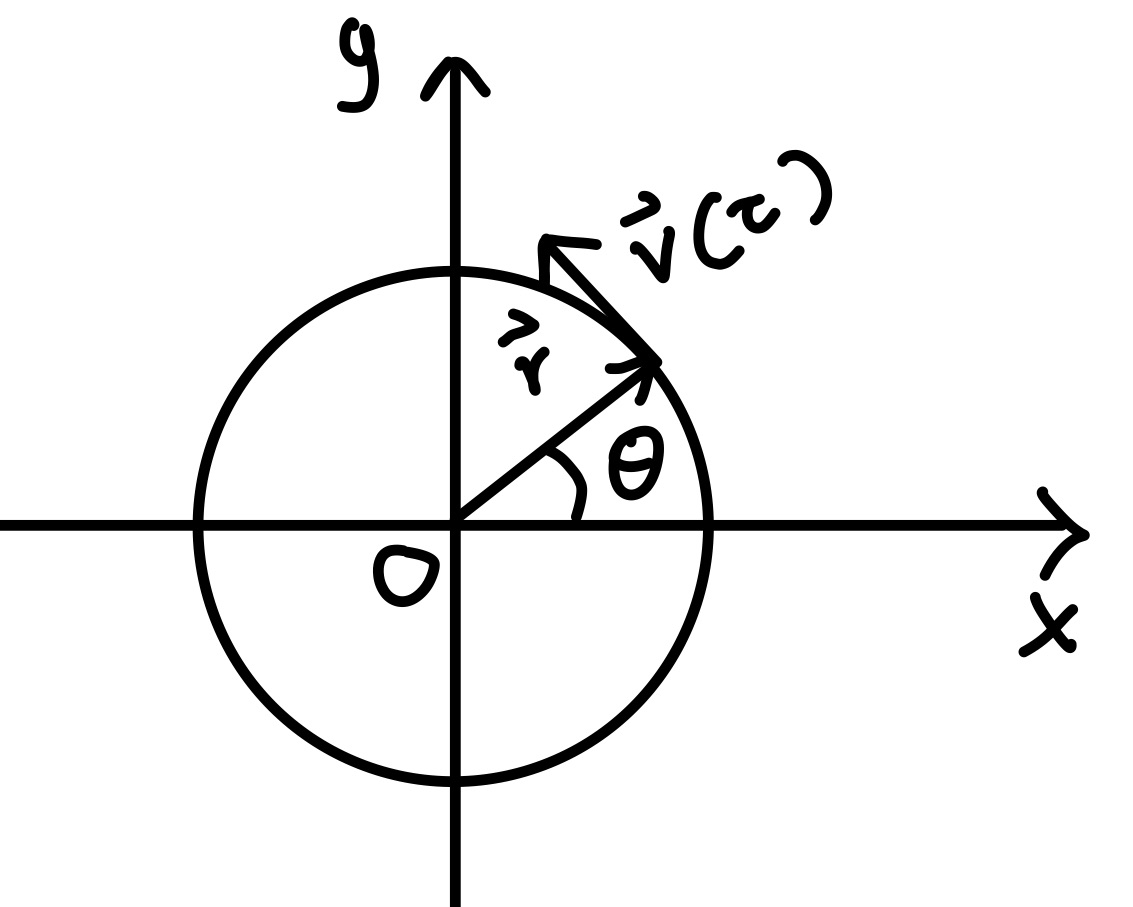
\includegraphics[scale=0.15]{grafico_3}
	\end{center}
	\[
	\overrightarrow{v} \overrightarrow{\omega}_r\times \overrightarrow{r}
	.\] 
	\[
		|\overrightarrow{\omega}_r| = \frac{d \theta}{dt} = \omega (t)
	.\] 
	\[
	\overrightarrow{a} = \overrightarrow{a}_t + \overrightarrow{a}_c
	.\]
	\[
		\overrightarrow{a}_t = \frac{d v(t)}{dt}\hat v + \overrightarrow\omega_v\times \overrightarrow{v} = a(t) = \alpha(t)r\hat v(t) = \overrightarrow{\alpha}(t)\times \overrightarrow{r}(t)
	.\] 
	\textbf{Accelerazione Centripeta}
	\[
	\overrightarrow{a_c}(t) = \overrightarrow{\omega}(t)\times \overrightarrow{v}(t) = \overrightarrow{\omega}(t)\times(\overrightarrow{\omega}(t)\times \overrightarrow{r}(t))
	.\] 
	\begin{center}
		
	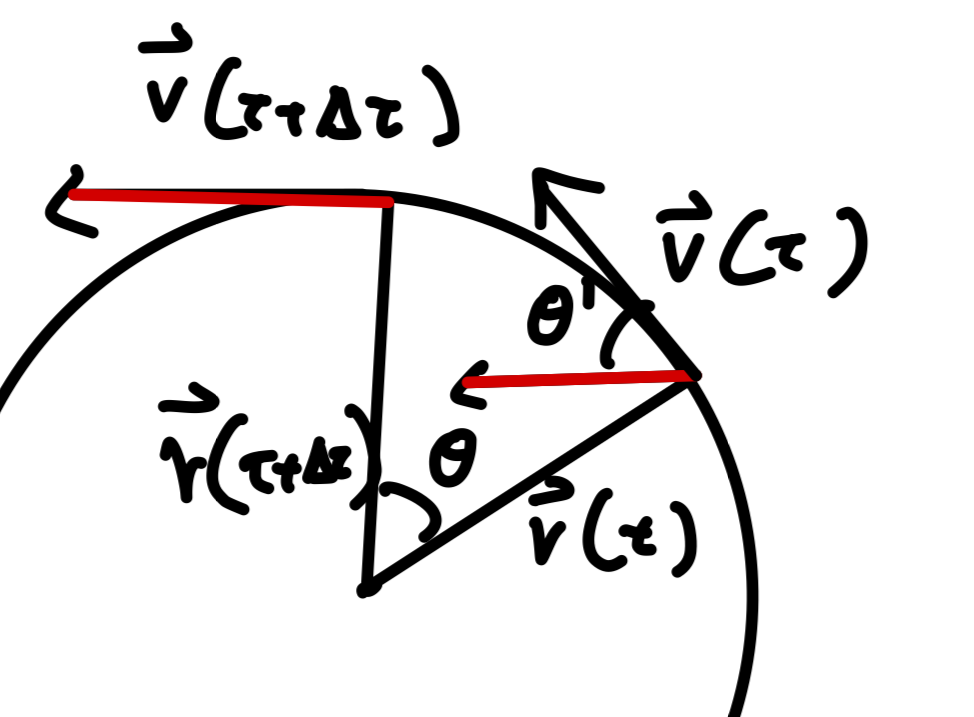
\includegraphics[scale=0.2]{grafico_4}
	\end{center}
	Dove $\theta'$ è l'angolo tra il corrente vettore della velocità e quello dopo  $\Delta t$
	\[
	| \overrightarrow{\omega}| = \omega (t)
	.\] 
	\[
	| \overrightarrow{v}(t)| = r \omega (t)
	.\] 
	\[
	| \overrightarrow{a}| = r \omega^2(t)
	.\] 
	\textbf{Velocità angolare}\\
	\[
		\omega (t) = \frac {d\theta(t)}{dt}
	.\] 
	\[
		\theta(t) = \frac {S_(t)}{r}
	.\] 
	Dove S(t) è l'ascissa curvilinea\\
	\begin{center}
	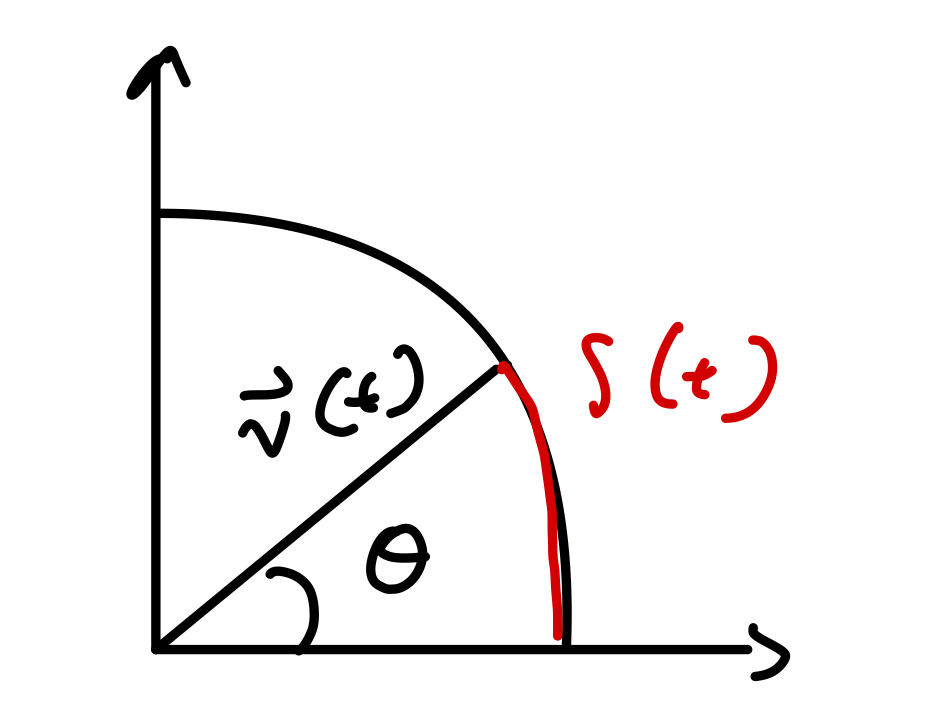
\includegraphics[scale=0.3]{grafico_5}
	\end{center}
	\[
		\frac{ dS(t)}{dt} = \lim_{\Delta t \rightarrow 0} = \frac{S(t)}{\Delta t} = \frac {d\theta}{dt} r
	.\] 
	\[
		a(t) = \frac{dv(t)}{dt} = \frac{d^2\theta(t)}{dt^2}r
	.\] 
	\textbf{Nota:}\\
	\begin{center}
		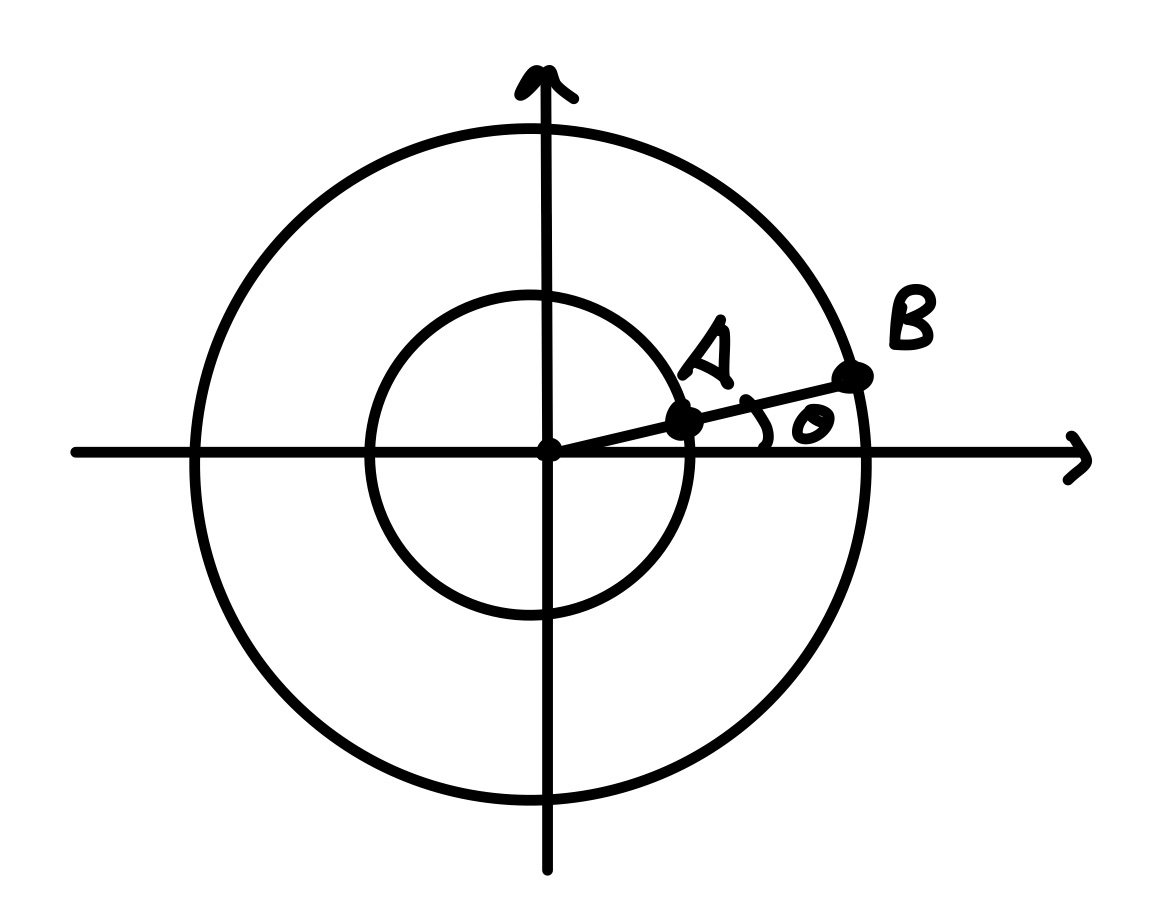
\includegraphics[scale=0.1]{grafico_6}
	\end{center}
L'accelerazione angolare è uguale nel punto materiale in $A$ e in $B$\\

\end{document}
